%% Related Work
%%=========================================

\chapter{Related Work}
\label{ch:related_work}
This chapter looks closer at related work carried out in the field of machine translation. We present the history and progress of machine translation in Section \ref{sec:natural_language_processing}. In section \ref{sec:statistical_machine_translation} we present statistical machine translation, and neural machine translation is presented in Section \ref{sec:neural_machine_translation}. We both present some early work and establish the current state-of-the-art in the field.

%%=========================================

\section{Evolution of Machine Translation}
\label{sec:natural_language_processing}
In 1954, a translation system developed at Georgetown University was demonstrated for the first time. The system did a completely automatic translation of more than sixty sentences from Russian to English. One of the creators, Léon Dostert, predicted that automatic text-reading translations machines would be finished within three to five years \citep{hutchins1997first}. As research continued, the complexity of the linguistic problems became more and more apparent. Critics argued that the concept of fully automatic high-quality translations that could produce translations indistinguishable from those of humans translators were impossible in principle \citep{hutchins2007machine}. 

National Science Foundation established the Automatic Language Processing Advisory Committee (ALPAC) in 1964 to carry out a study of the realities of machine translation. In 1966 they published their report that concluded that the use of machine translation was slower, less accurate, and twice as expensive as human translation. The report also stated that there were no immediate or predictable prospect of useful machine translation \citep{hutchins2007machine, national1966language, koehn2010statistical}. The ALPAC report led to the U.S government reducing their funding in the field dramatically.

It was first in the later half of the 1970s, and the early 1980s, that machine translation again saw a rise in popularity. The latter half of the 1980s also saw a general revival in interest in Interlingua systems. This interest was motivated in part by artificial intelligence, which was also a research field that attracted much attention. Since the 1980s, new methods such as corpus-based approaches and statistical machine translation based systems has emerged. Speech translation has also seen growing interest since the late 1980s \citep{hutchins2007machine}.

\begin{figure}[H]
    \centering
    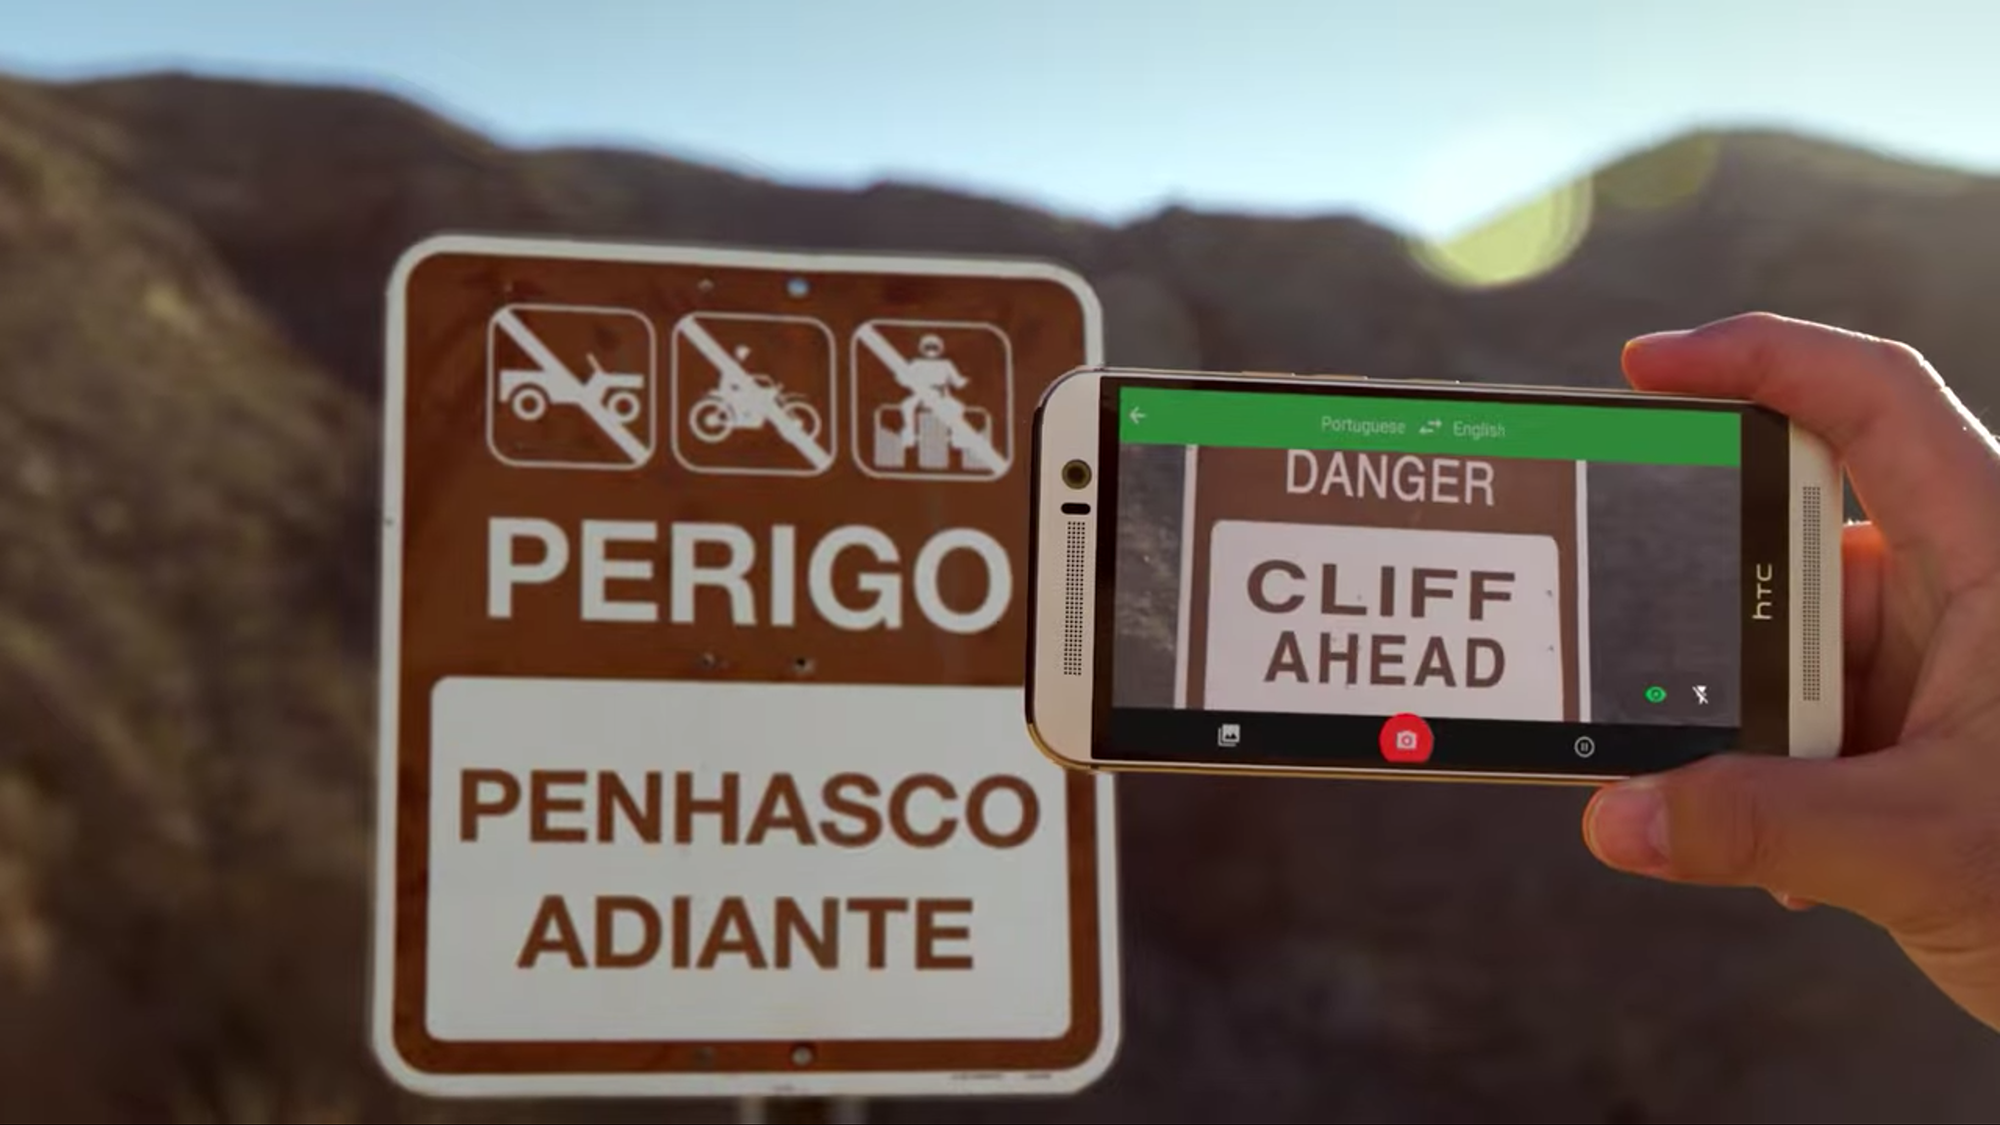
\includegraphics[width=0.8\textwidth]{fig/background_theory/google_translate_rt.png}
    \caption{The Google Translate app and its image translation feature}
    \label{fig:google-translate-rt}
\end{figure}

In more recent years, online solutions such as Google Translate\footnote{https://translate.google.com} and Yahoo!'s Babelfish\footnote{https://www.babelfish.com}\footnote{The service now relies on the translations from the Bing Translator, but the service is otherwise unaltered} has gained much popularity. Both services offer on-demand translation for free \citep{schuster2016googletranslate, hutchins2007machine}. Google reported on their blog in 2016 that their service supported over 100 languages, had more than 500 million users, and translated more than 100 billion words a day \citep{turovsky2016googletranslate}. The native app for Google Translate has also become very popular. It offers the same functionality as their online counterpart, but also offer a few additional features, such as ``Word Lens'' which translates images in place (see Figure \ref{fig:google-translate-rt}).

%%=========================================

\section{Statistical Machine Translation}
For the past two decades or so, machine translation has taken a new direction. Instead of pre-defined rule-based systems, many modern machine translation systems attack the problem of machine translation with statistical methods and ideas from information theory \citep{brown1990statistical}. Statistical machine translation was born as an idea in the 1980s in the labs of IBM Research. The idea came in the wake of the success of statistical methods in speech recognition. The idea was to model the translation task as a statistical optimization problem. Some of the best performing SMT systems today are phrase-based, an approach where the input sequence is broken up into a sequence of phrases, and these phrases are mapped one-to-one to output phrases, which may be reordered \citep{koehn2010statistical}. See Figure \ref{fig:translation-phrase-based} for illustration of a phrase-based translation of a sentences in German to English.

\label{sec:statistical_machine_translation}
\begin{figure}[ht]
    \centering
    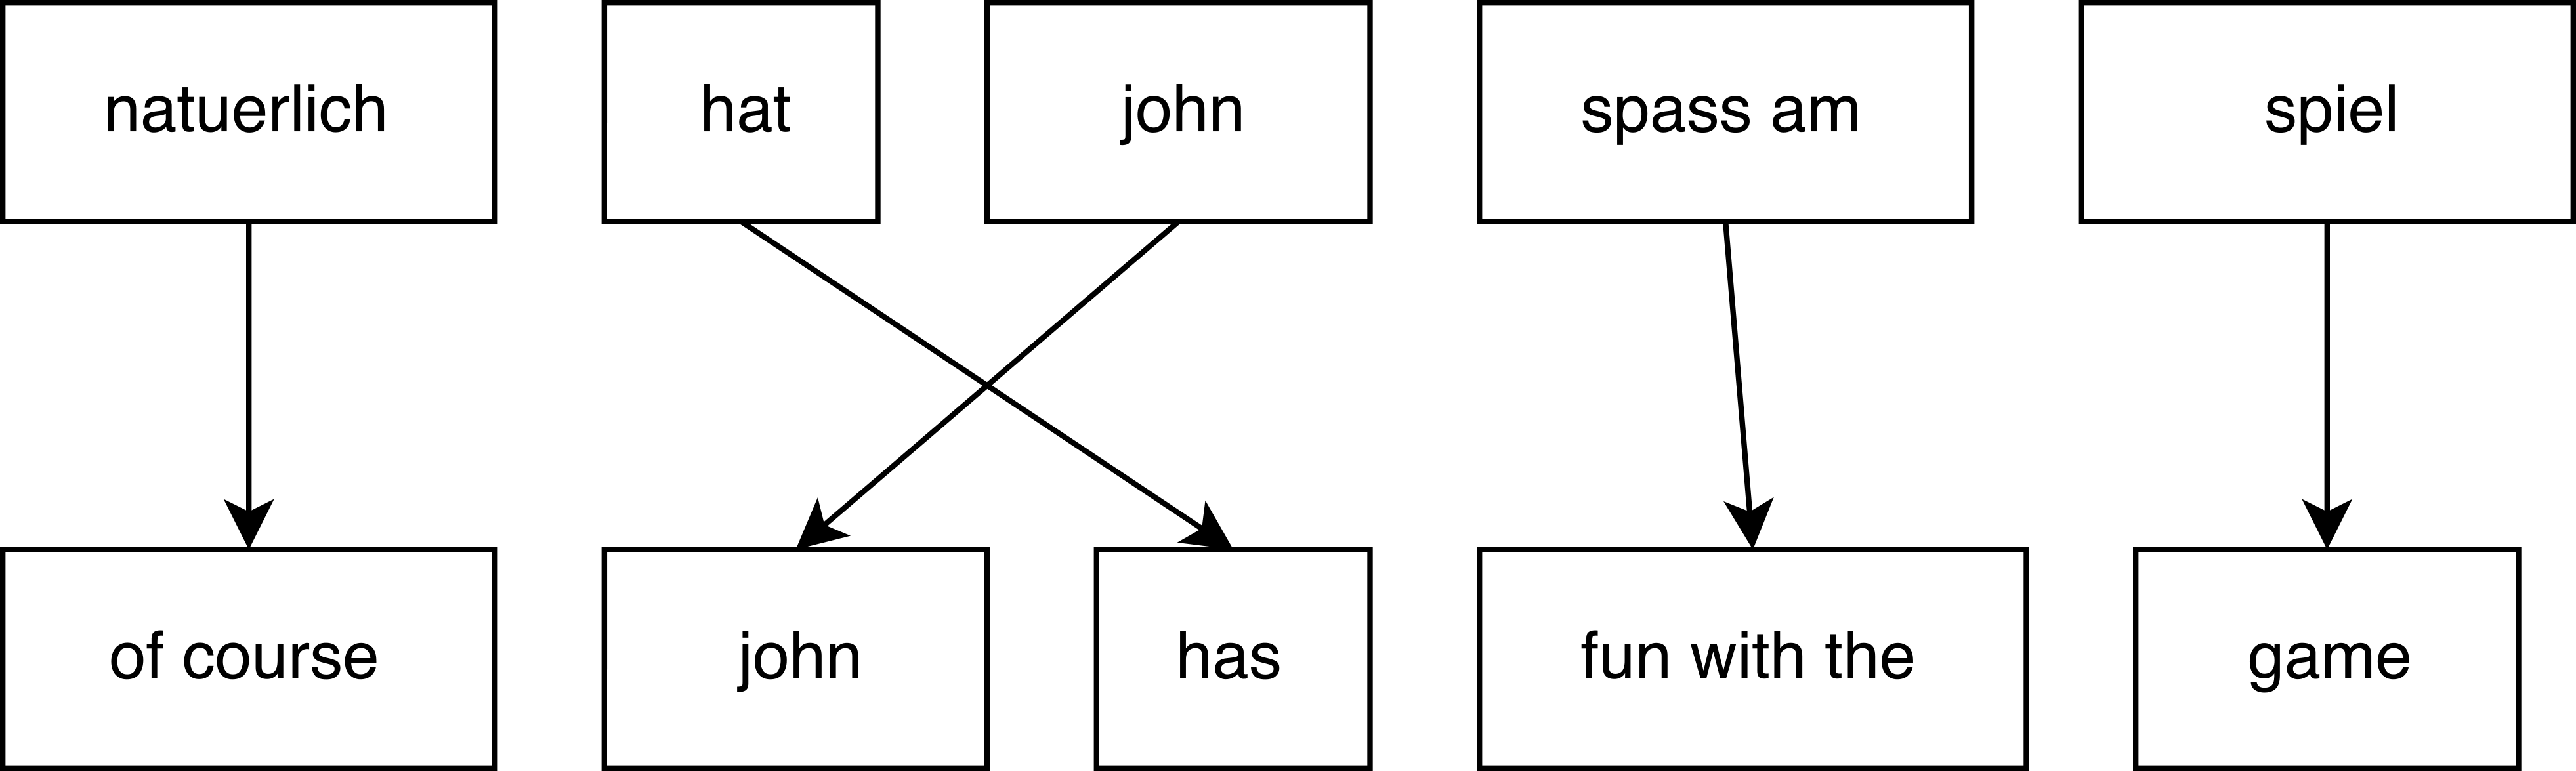
\includegraphics[width=0.8\textwidth]{fig/related_work/translation.png}
    \caption{Phrase-based translation of a sentence in German to English}
    \label{fig:translation-phrase-based}
\end{figure}

Statistical machine translation has been the dominant translation paradigm for decades \citep{wu2016google}. Variants and implementations of SMT-based systems have achieved state-of-the-art performance in machine translation \citep{watanabe07onlinelargemargin}. SMT system also exist on the commercial market, a market long dominated by the well-established, and older, rule-based methods \citep{hutchins2007machine}.

%%=========================================

\section{Neural Machine Translation}
\label{sec:neural_machine_translation}
Neural machine translation is another approach to machine translation that has emerged recently. This approach aims at building a jointly-tuned single neural network which is trained to maximize translation performance. This is a different approach from traditional statistical machine translation systems, where a translation system consists of sub-components that are optimized separately \citep{wolk2015neural}. The benefit of neural machine translation systems is its ability to learn directly, in an end-to-end fashion. 

In 2016, Google published their work on Google's Neural Machine Translation system, or GNMT for short. This system replaced their older statistical machine translation system that ran Google Translate \citep{turovsky2016googletranslatenmt}. GNMT uses the common sequence-to-sequence learning framework as proposed by \cite{sutskever2014sequence, wu2016google}. Their implementation is closely related to the work of \cite{kalchbrenner2013recurrent} who were the first to map the input sentence into a vector, and then back into a sentence using the encoder-decoder framework. It also builds on the neural network architecture presented by \cite{cho2014learning}. \cite{cho2014learning} did their translation using LSTM-like RNN architecture, although their primary focus was to integrate their neural network into an SMT system \citep{cho2014learning, sutskever2014sequence}. The proposed model of \cite{sutskever2014sequence} did the entire translation end-to-end and was not integrated with any other frameworks or systems. Their implementation achieved close-to-best results in an English to French translation task and outperformed various SMT-based systems.

\begin{figure}[ht]
    \centering
    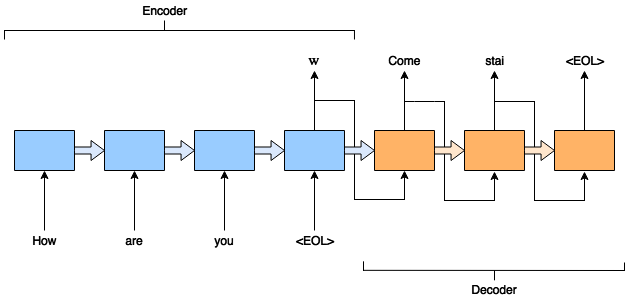
\includegraphics[width=0.8\textwidth]{fig/related_work/encoder_decoder_en_it.png}
    \captionsetup{justification=centering}
    \caption{General translation approach in neural machine translation from an English sentence to Italian}
    \label{fig:machine-translation-encoder-decoder-simple}
\end{figure}

The encoder-decoder approach, as shown in Figure \ref{fig:machine-translation-encoder-decoder-simple} has also been used as the foundation for various other NMT architectures. \cite{chung2016character} used the encoder-decoder general approach in their experiment, GRUs, instead of LSTMs, with their model dubbed \emph{bi-scale recurrent neural network}, which handled better multiple timescales in a sequence. Their model did the translation on character-level instead of the more common approach of translating on word-level. They proved that their decoder, which was fed sequences of characters without any explicit word segmentation, was able to translate at the level of characters, and that the model benefited from the approach. 

\cite{bahdanau2014neural} proposed another model, as already introduced in Section \ref{sec:attention_mechanism}, which tried to solve the performance bottleneck related to the encoded vector. \cite{cho2014properties} had already shown that the encoder-decoder model had problems with longer dependencies. Their analysis also introduced a novel network dubbed \textit{gated recursive convolutional neural network}, which was evaluated alongside the more traditional encoder-decoder approach. Their evaluation showed that both architectures performed relatively well on short sentences, but suffered significantly as the length of the sentences increased. The model proposed by \cite{bahdanau2014neural} instead learns to align and translate jointly. It does this by encoding the input sequence into a sequence of vectors and chooses a subset of these vectors adaptively while decoding the translation. This model outperformed the basic encoder-decoder significantly in their experiments.

Despite being a relatively new approach, neural machine translation has achieved impressive results. In many machine translation tasks, they have obtained state-of-the-art performance, outperforming statistical machine translation systems that have matured over several decades. \cite{bahdanau2014neural} stated that most of the proposed neural network translation models belonged to a family of encoder-decoders, making it the key factor for this success in many models. Recently, new work has been published that addresses other problems and bottlenecks with the encoder-decoder architecture, such as the rare word problem, increasing performance even further \citep{sennrich2015neural}. The attention mechanism has also shown promising results since it was first introduced, achieving new state-of-the-art results in certain translation tasks \citep{luong2015effective}.